\documentclass[conference]{IEEEtran}
\IEEEoverridecommandlockouts

\usepackage{amsmath,amssymb,amsfonts}
\usepackage{algorithmic}
\usepackage{graphicx}
\usepackage{textcomp}
\usepackage{xcolor}
\usepackage{booktabs}
\usepackage{cite}
\usepackage{url}
\usepackage{microtype}
\usepackage{listings}

\lstset{
  basicstyle=\ttfamily\footnotesize,
  breaklines=true,
  frame=single,
  backgroundcolor=\color{gray!10}
}

\begin{document}

\title{SemanticSync: Schema-Level Semantic Merge Policies for Local-First Relational Databases}

\author{
\IEEEauthorblockN{Pathak Ashmit Akhilesh}
\IEEEauthorblockA{\textit{Department of Computer Science and Engineering} \\
\textit{Vellore Institute of Technology}\\
Vellore, India \\
pathak.ashmit2025@vitstudent.ac.in}
\and
\IEEEauthorblockN{Yash Bohra}
\IEEEauthorblockA{\textit{Department of Computer Science and Engineering} \\
\textit{Vellore Institute of Technology}\\
Vellore, India \\
yash.bohra2025@vitstudent.ac.in}
}

\maketitle

\begin{abstract}
Local-first software lets client devices read and write local data while offline, then sync when connected. While Conflict-Free Replicated Data Types (CRDTs) guarantee mathematical convergence for specific data structures, naive syntactic policies like Last-Writer-Wins often discard business intent and break relational constraints. We present SemanticSync, a replication and merge middleware built for local-first SQLite databases. SemanticSync provides schema-assigned pairwise merge policies (\texttt{SUM}, \texttt{BOUNDED\_SUM}, \texttt{AVG}, \texttt{APPEND}, \texttt{LWW}, \texttt{MIN}, \texttt{MAX}, and \texttt{REJECT}), explicit numeric \texttt{INCREMENT} tracking, non-destructive foreign-key orphan quarantine, and checkpoint-assisted causal log compaction. We evaluated the engine across two benchmark suites: a historical state-based stress workload and a 90-trial explicit-\texttt{INCREMENT} matrix across 1,000, 5,000, and 10,000 operations at 5\%, 20\%, and 50\% conflict densities. Across all 90 validated trials, SemanticSync achieved 100.0\% Semantic Correctness Rate (SCR) and 100.0\% Benchmark-Row Value Agreement (RVAR) against an arithmetic oracle, whereas Last-Writer-Wins scored 0.0\% SCR by discarding concurrent deltas. Batch synchronization incurred measurable timing differences compared to an uninstrumented SQL baseline (median deltas from 449.7~ms to 84,368.7~ms), reflecting the concrete cost of operation logging, receipt tracking, and foreign-key checks.
\end{abstract}

\begin{IEEEkeywords}
Local-first software, SQLite replication, semantic merge policies, conflict resolution, referential integrity, causal log compaction.
\end{IEEEkeywords}

\section{Introduction}

\subsection{The Local-First Relational Dilemma}
Local-first computing gives users local ownership and instant access to their data without continuous cloud access~\cite{kleppmann2019localfirst}. Devices work offline and sync when connected. This model is attractive, but relational databases complicate it. Relational applications rely on primary and foreign keys. Local updates carry specific business rules. When disconnected replicas sync after hours or days of network isolation, simple reconciliation mechanisms break down.

Pioneering CRDT research establishes strong eventual consistency for primitive data structures~\cite{shapiro2011crdt, gomes2017verifying}. However, converging to an identical state is not the same as being correct. In relational applications, picking a single winner across conflicting updates silently discards user intent and violates domain rules.

\subsection{The Convergence vs. Correctness Paradox}
To see why syntactic convergence falls short of semantic correctness, consider an inventory table:
\begin{lstlisting}[language=SQL]
CREATE TABLE inventory (
    item_id INTEGER PRIMARY KEY,
    quantity INTEGER
);
\end{lstlisting}
Suppose item~1 starts with a stock of 100 in the common ancestor state. While disconnected, two store replicas record independent sales:
\begin{itemize}
    \item Replica A sells 15 units: \texttt{UPDATE inventory SET quantity = 85 WHERE item\_id = 1;}
    \item Replica B sells 20 units: \texttt{UPDATE inventory SET quantity = 80 WHERE item\_id = 1;}
\end{itemize}

Under a standard Last-Writer-Wins (LWW) rule~\cite{dynamo2007}, the replica with the higher timestamp wins. If Replica~B has the later timestamp, both databases converge to 80 units. The databases match, but 15 sold units simply vanish. The true inventory reflecting both transactions is 65 units.

Similar failures happen across other domains:
\begin{itemize}
    \item \textit{Collaborative sensing:} Averaging sensor readings (\texttt{AVG}) or appending clinical notes (\texttt{APPEND}) fails when one writer overwrites another.
    \item \textit{Security and access control:} Edits to user roles or patient blood types should never be resolved by timestamps. They require human intervention (\texttt{REJECT}).
    \item \textit{Referential integrity:} Deleting a parent row while another replica inserts a child row leaves orphan rows or triggers foreign-key constraint panics.
\end{itemize}

\subsection{Contributions}
We built SemanticSync to bridge the gap between syntactic convergence and domain correctness. Our main contributions are:
\begin{enumerate}
    \item \textbf{Schema-assigned pairwise policies:} A type-safe framework that binds merge policies (\texttt{SUM}, \texttt{BOUNDED\_SUM}, \texttt{AVG}, \texttt{APPEND}, \texttt{LWW}, \texttt{MIN}, \texttt{MAX}, \texttt{REJECT}) directly to table columns.
    \item \textbf{Tracked explicit-INCREMENT model:} An operation-logging model that separates absolute state overwrites from additive numeric increments, preventing duplicate replay with stable receipts.
    \item \textbf{Foreign-key quarantine protocol:} A protocol that moves dependent child rows into \texttt{\_ss\_quarantine} before parent deletion, keeping \texttt{PRAGMA foreign\_keys = ON} active throughout.
    \item \textbf{Checkpoint log compaction:} A pruning protocol that checks acknowledgment vectors, replica membership, and snapshot integrity before trimming the operation log.
    \item \textbf{Empirical evaluation:} A 90-trial matrix spanning 1,000 to 10,000 operations at varying conflict densities, measuring correctness, replica agreement, and sync overhead.
\end{enumerate}

\section{System Architecture}

We built SemanticSync as an embeddable middleware between local application SQL execution and replication channels (Fig.~\ref{fig:arch}). The engine sits alongside SQLite on each client device, intercepting writes and managing sync sessions.

\begin{figure*}[!t]
\centering
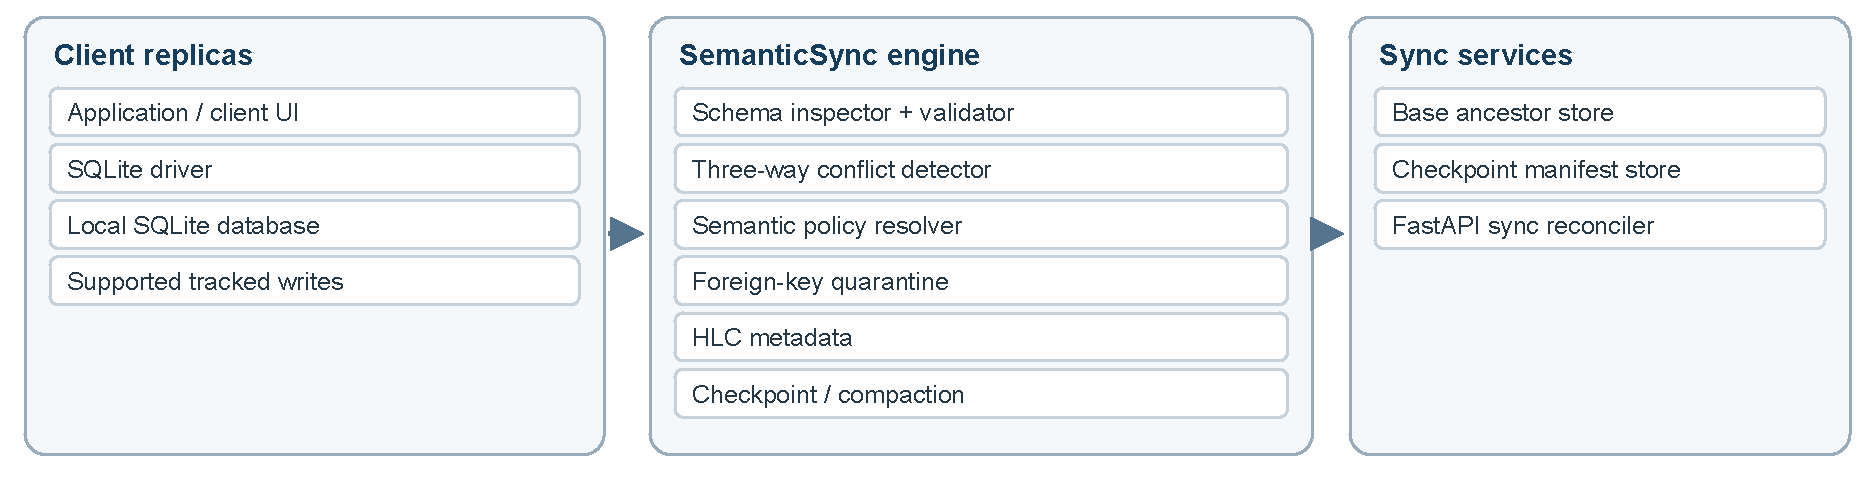
\includegraphics[width=0.92\textwidth]{fig1_architecture.pdf}
\vspace{-2mm}
\caption{SemanticSync architectural layers, showing how tracked replica mutations pass through schema inspection, conflict detection, semantic resolution, and quarantine management.}
\label{fig:arch}
\vspace{-2mm}
\end{figure*}

\subsection{Storage Layout and Tracked Operation Log}
Each local SQLite replica holds user tables and four internal metadata tables:
\begin{itemize}
    \item \texttt{\_ss\_change\_log}: Stores local and received column mutations (\texttt{table\_name}, \texttt{row\_id}, \texttt{column\_name}, \texttt{old\_value}, \texttt{new\_value}, \texttt{ts\_pt}, \texttt{ts\_l}, \texttt{replica\_id}, \texttt{op\_type}, \texttt{origin\_id}, \texttt{sequence}, \texttt{source\_id}, \texttt{depends\_on}, \texttt{bounded\_delta}, \texttt{bounds\_min}, \texttt{bounds\_max}).
    \item \texttt{\_ss\_quarantine}: Holds child rows isolated during parent deletions (\texttt{quarantine\_id}, \texttt{table\_name}, \texttt{row\_id}, \texttt{row\_payload}, \texttt{parent\_table}, \texttt{parent\_row\_id}, \texttt{reason}, \texttt{quarantined\_at}, \texttt{status}).
    \item \texttt{\_ss\_compacted\_receipts}: Records hashes and IDs of compacted entries to catch and discard duplicate deliveries.
    \item \texttt{\_ss\_checkpoint\_metadata}: Tracks checkpoint incarnation IDs and snapshot epochs.
\end{itemize}

We separate absolute \texttt{SET}/\texttt{UPDATE} operations from numeric \texttt{INCREMENT} operations. When an application calls \texttt{apply\_increment}, the engine assigns a unique \texttt{origin\_id} and records the signed delta. During sync, incoming increments apply once and record a stable receipt in the change log. This stops replay attacks and duplicate delivery. The design borrows concepts from operation-based CRDTs~\cite{bauwens2023} by syncing small deltas instead of entire rows, saving network bandwidth. However, SemanticSync does not claim general CRDT convergence across arbitrary topologies. Its guarantees apply strictly to pairwise synchronizations.

\subsection{Hybrid Logical Clocks}
To order operations without synchronized physical clocks, we use Hybrid Logical Clocks (HLC)~\cite{hlc2014}. Each replica tracks physical time $pt$, a logical counter $l$, and samples the local wall clock $pt_{\text{wall}}$. On a local write, if $pt_{\text{wall}} > pt_{\text{local}}$, the clock advances to $(pt_{\text{wall}}, 0)$; otherwise, it increments the logical counter to $(pt_{\text{local}}, l_{\text{local}} + 1)$. When receiving an operation with timestamp $(pt_{\text{msg}}, l_{\text{msg}})$, the clock updates as follows:
\begin{equation}
pt' = \max(pt_{\text{local}}, pt_{\text{msg}}, pt_{\text{wall}}),
\end{equation}
\begin{equation}
l' = \begin{cases} 
\max(l_{\text{local}}, l_{\text{msg}}) + 1 & \text{if } pt' = pt_{\text{local}} = pt_{\text{msg}} \\ 
l_{\text{local}} + 1 & \text{if } pt' = pt_{\text{local}} \\ 
l_{\text{msg}} + 1 & \text{if } pt' = pt_{\text{msg}} \\ 
0 & \text{otherwise } (pt' = pt_{\text{wall}}) 
\end{cases}
\end{equation}
The logical counter advances whenever the physical clock fails to jump strictly ahead of prior timestamps. It resets to zero only when the local wall clock catches up and overtakes them. These HLC timestamps provide deterministic tie-breaking for timestamped policies, though they do not replace causal vector clocks in full mesh networks.

\section{Semantic Merge Policy Framework}

\subsection{Mathematical Formalization}
Let $\mathcal{V}$ denote attribute values, and let $\mathcal{M}$ represent operation metadata (replica ID, HLC timestamp, and operation identity). A three-way semantic resolution function $\mathcal{R}$ maps these inputs:
\begin{equation}
\mathcal{R}: \mathcal{V} \times (\mathcal{V} \times \mathcal{M}) \times (\mathcal{V} \times \mathcal{M}) \to \mathcal{V} \cup \{\bot\}
\end{equation}
Here, $\bot$ indicates an unresolved conflict flagged for manual review.

Pairwise merge symmetry requires that swapping the two replica inputs produces the same result:
\begin{equation}
\begin{aligned}
\mathcal{R}(v_{\text{base}}, (v_A, m_A), (v_B, m_B)) = \\
\mathcal{R}(v_{\text{base}}, (v_B, m_B), (v_A, m_A))
\end{aligned}
\end{equation}

\subsection{Supported Semantic Policies}
SemanticSync implements eight schema-level merge policies (Table~\ref{tab:policies}).

\begin{table*}[!t]
\centering
\footnotesize
\setlength{\tabcolsep}{4pt}
\caption{Implemented Semantic Merge Policies and Tested Properties}
\label{tab:policies}
\begin{tabular}{p{0.15\textwidth}p{0.18\textwidth}p{0.27\textwidth}p{0.32\textwidth}}
\toprule
\textbf{Policy} & \textbf{Compatible Types} & \textbf{Resolution Semantics} & \textbf{Algebraic Properties \& Boundaries} \\
\midrule
\texttt{SUM} & Numeric (\texttt{INT, REAL}) & $v_{\text{base}} + (v_A - v_{\text{base}}) + (v_B - v_{\text{base}})$ & Commutative for fixed base; delta addition associative; non-idempotent. \\
\texttt{BOUNDED\_SUM} & Numeric (\texttt{INT, REAL}) & Delta checked against $[\min, \max]$; flags $\bot$ if out of bounds & Invariant-preserving; rejects unsafe candidate states without clamping. \\
\texttt{AVG} & Numeric (\texttt{INT, REAL}) & $(v_A + v_B) / 2.0$ & Commutative; strictly non-associative; suitable for pairwise sensor merges. \\
\texttt{APPEND} & Text (\texttt{TEXT}) & Concatenates text ordered by replica ID & Pairwise commutative; lacks element-level identity; not arbitrary $N$-way join. \\
\texttt{LWW} & Any SQLite type & Higher HLC timestamp wins; ties broken by replica ID & Syntactically deterministic; disregards business semantics. \\
\texttt{MIN} / \texttt{MAX} & Numeric types & $\min(v_A, v_B)$ or $\max(v_A, v_B)$ & Commutative, associative, idempotent (semilattice). \\
\texttt{REJECT} & Any SQLite type & Emits $\bot$ (flagged for review) & Safety stop preventing automated silent overwrites. \\
\bottomrule
\end{tabular}
\end{table*}

\subsection{Tombstone Reconciliation (Update vs. Delete)}
When one replica updates a row while another deletes it, SemanticSync flags an \texttt{UPDATE\_DELETE} conflict. Concurrent update-remove conflicts present a classic dilemma in distributed systems~\cite{removewin2021}. Rather than imposing a single theoretical rule, SemanticSync lets developers configure one of three strategies:
\begin{itemize}
    \item \texttt{DELETE\_WINS}: Deletion takes precedence. The row is removed and the concurrent update is dropped.
    \item \texttt{UPDATE\_RESURRECTS}: The update takes precedence. The row is kept with its updated values.
    \item \texttt{FLAG\_FOR\_REVIEW}: The conflict moves to \texttt{MergeManager} for manual inspection.
\end{itemize}

\subsection{Type Compatibility and Validation}
Before assigning a policy, our \texttt{PolicyValidator} inspects SQLite column affinities using \texttt{PRAGMA table\_info}. If an invalid binding is attempted, such as setting \texttt{SUM} on a \texttt{TEXT} column, the engine rejects it immediately with HTTP 422 Unprocessable Entity. This fail-fast check catches configuration mistakes at startup.

\section{Foreign-Key Quarantine Boundary}

In relational systems, multi-master replication easily violates referential integrity. In SQLite, referential constraints require \texttt{PRAGMA foreign\_keys = ON}.

\subsection{The Referential Cascade Problem}
Consider a parent table \texttt{departments(dept\_id)} and a child table \texttt{employees(emp\_id, dept\_id)}. Suppose Replica~A deletes a department while Replica~B inserts or modifies an employee in that department. Standard replication runs into a dead end:
\begin{enumerate}
    \item Replaying the department deletion on Replica~B triggers a foreign-key error (\texttt{sqlite3.IntegrityError}).
    \item Turning off foreign keys (\texttt{PRAGMA foreign\_keys = OFF}) leaves corrupt orphan rows in the database.
\end{enumerate}

\subsection{Quarantine Isolation Protocol}
To keep referential integrity intact without losing data, we built an atomic orphan quarantine protocol:
\begin{enumerate}
    \item \textbf{Connection enforcement:} Every database connection enables \texttt{PRAGMA foreign\_keys = ON} before running transactions.
    \item \textbf{Dependency introspection:} Before deleting a parent row from table $T$ with primary key $K$, the engine runs \texttt{PRAGMA foreign\_key\_list} across user tables to spot referencing child rows.
    \item \textbf{Atomic quarantine:} The engine copies any referencing child rows into \texttt{\_ss\_quarantine} as JSON payloads, together with parent references and timestamps.
    \item \textbf{Child and parent deletion:} The engine deletes child rows first, then deletes the parent row. Foreign keys remain satisfied throughout.
    \item \textbf{Post-validation:} Before calling \texttt{COMMIT}, the transaction runs \texttt{PRAGMA foreign\_key\_check}. Any violation rolls back the entire batch.
    \item \textbf{Operator restoration:} Operators can view quarantined rows via \texttt{GET /api/v1/quarantine} and either reassign them to a new parent (\texttt{POST /api/v1/quarantine/\{id\}/resolve}) or delete them permanently.
\end{enumerate}

\section{Checkpoint-Assisted Log Compaction}

Logging every mutation causes SQLite databases to grow indefinitely and slows down sync replay. To prune historical logs safely, we implemented a checkpoint protocol.

\subsection{Compaction Eligibility Checks}
Pruning an entry too early can permanently strand a disconnected replica. SemanticSync only prunes an operation when all of the following conditions hold:
\begin{enumerate}
    \item \textbf{Unanimous acknowledgment:} The operation ID must be acknowledged by all enrolled replicas.
    \item \textbf{Payload hash match:} The SHA-256 hash of the operation payload must match across all replica receipts.
    \item \textbf{Stable horizon cutoff:} The cutoff timestamp $H_{\text{stable}}$ is the minimum of the highest acknowledged HLC timestamps across all replicas:
    \begin{equation}
    H_{\text{stable}} = \min_{r \in \mathcal{R}} \left( \max_{op \in \text{ACK}_r} \text{HLC}(op) \right)
    \end{equation}
    Only operations with $\text{HLC} < H_{\text{stable}}$ can be pruned.
    \item \textbf{Dependency closure:} An operation cannot be pruned if any active change-log entry depends on it.
\end{enumerate}

\subsection{Atomic Pruning Execution}
During a \texttt{BEGIN IMMEDIATE} transaction, eligible entries are deleted from \texttt{\_ss\_change\_log}. At the same time, compact receipt records are inserted into \texttt{\_ss\_compacted\_receipts}. If an out-of-date peer later sends a pruned operation, the engine checks \texttt{\_ss\_compacted\_receipts} and drops the duplicate without error.

\section{Empirical Evaluation}

We evaluated SemanticSync across two benchmark suites:
\begin{enumerate}
    \item \textbf{Historical SET-based stress benchmark:} A state-diffing workload with 1,000, 5,000, and 10,000 operations at 5\%, 20\%, and 50\% conflict densities (two paired trials per cell).
    \item \textbf{Explicit-INCREMENT evaluation matrix:} A 90-trial matrix auditing dedicated operation-based increments across nine configurations (10 independent seeds per cell), following standard synthetic CRDT benchmark designs~\cite{crust2025}.
\end{enumerate}

All benchmarks ran on a single Windows 11 host (Python 3.14.3, SQLite 3.50.4, \texttt{journal\_mode = DELETE}).

\subsection{Evaluation Metrics}
\begin{itemize}
    \item \textbf{Semantic Correctness Rate (SCR):} The percentage of conflict rows matching the arithmetic oracle ($v_{\text{expected}} = v_{\text{base}} + \Delta_A + \Delta_B$), evaluated across both replicas ($2 \times C$ observations per trial).
    \item \textbf{Benchmark-Row Value Agreement (RVAR):} The percentage of matching \texttt{bench\_rows.value} entries across both replicas, measuring replica convergence.
    \item \textbf{Valid Resolution Accuracy (VRA):} The percentage of values satisfying domain constraints (unmeasured in synthetic runs lacking domain rules).
    \item \textbf{Paired Timing Difference:} The synchronization time difference between SemanticSync and the baseline: $\Delta = T_{\text{engine}} - T_{\text{baseline}}$.
\end{itemize}

\subsection{Historical SET-Based Evaluation Results}
In the state-based benchmark (Table~\ref{tab:set_stress} and Table~\ref{tab:set_timing}), SemanticSync reached SCR scores between 97.50\% and 98.25\%. In contrast, LWW scored 0.00\% against the additive oracle.

\begin{table}[!t]
\centering
\caption{Historical SET-Based Repeated Stress Measurements (2 Paired Trials per Cell)}
\label{tab:set_stress}
\begin{tabular}{rrrrr}
\toprule
\textbf{Operations} & \textbf{Density} & \textbf{LWW SCR} & \textbf{Sync SCR} & \textbf{RVAR} \\
\midrule
1,000 & 5\% & 0.0\% & 98.0\% & 100.0\% \\
1,000 & 20\% & 0.0\% & 97.5\% & 100.0\% \\
1,000 & 50\% & 0.0\% & 98.2\% & 100.0\% \\
5,000 & 5\% & 0.0\% & 98.0\% & 100.0\% \\
5,000 & 20\% & 0.0\% & 98.0\% & 100.0\% \\
5,000 & 50\% & 0.0\% & 98.2\% & 100.0\% \\
10,000 & 5\% & 0.0\% & 98.2\% & 100.0\% \\
10,000 & 20\% & 0.0\% & 98.2\% & 100.0\% \\
10,000 & 50\% & 0.0\% & 97.7\% & 100.0\% \\
\bottomrule
\end{tabular}
\end{table}

\begin{table}[!t]
\centering
\caption{Historical SET-Based Synchronization Durations and Paired Deltas}
\label{tab:set_timing}
\begin{tabular}{rrrr}
\toprule
\textbf{Ops} & \textbf{Density} & \textbf{LWW Median (s)} & \textbf{Paired $\Delta$ (ms)} \\
\midrule
1,000 & 5\% & 1.109 & +22.79 \\
1,000 & 20\% & 3.435 & -71.81 \\
1,000 & 50\% & 7.881 & -107.20 \\
5,000 & 5\% & 11.345 & -5.02 \\
5,000 & 20\% & 29.214 & +2,804.71 \\
5,000 & 50\% & 74.180 & +1,421.64 \\
10,000 & 5\% & 76.220 & -1,394.30 \\
10,000 & 20\% & 118.678 & +28,967.53 \\
10,000 & 50\% & 193.364 & -5,276.10 \\
\bottomrule
\end{tabular}
\end{table}

Auditing the data revealed why SemanticSync missed the remaining 2\%: when both replicas made the same non-base update independently ($v_A = v_B$), state diffing detected no divergence and applied nothing. But the additive oracle expected both changes ($v_{\text{base}} + 2\Delta$). This limitation in state-level diffing prompted us to build the explicit-\texttt{INCREMENT} model.

\subsection{Explicit-INCREMENT Evaluation Matrix}
To test the operation-based model, we ran a complete 9-configuration matrix with 10 independent trials per configuration (90 trials total).

Each configuration used 10 dedicated seeds: 1k/5\% (seeds 20263000--20263009), 1k/20\% (seeds 20263100--20263109), 1k/50\% (seeds 20263200--20263209), 5k/5\% (seeds 20263300--20263309), 5k/20\% (seeds 20263400--20263409), 5k/50\% (seeds 20263500--20263509), 10k/5\% (seeds 20263600--20263609), 10k/20\% (seeds 20263700--20263709), and 10k/50\% (seeds 20263800--20263809). Each trial created clean replica databases, applied local operations, and executed one batch sync.

We checked all trials using \texttt{research.experiments.validate\_increment\_evaluation}. Every trial passed without error. SQLite reported clean database integrity (\texttt{PRAGMA integrity\_check == ok}), change logs matched expected receipts ($N + C$ per replica), and final values showed zero error against the oracle.

\begin{table*}[!t]
\centering
\caption{Audited Explicit-INCREMENT Nine-Configuration Evaluation Matrix (10 Independent Seeds per Cell, 90 Trials Total)}
\label{tab:inc_matrix}
\begin{tabular}{rrrrrrc}
\toprule
\textbf{Operations} & \textbf{Conflict Density} & \textbf{Trials} & \textbf{SCR Summary} & \textbf{RVAR Summary} & \textbf{Median Paired $\Delta$ ($T_{\text{inc}} - T_{\text{app}}$)} & \textbf{IQR} \\
\midrule
1,000 & 5\% & 10 & 100.0\% (all trials) & 100.0\% (all trials) & 449.7 ms & 30.6 ms \\
1,000 & 20\% & 10 & 100.0\% (all trials) & 100.0\% (all trials) & 668.8 ms & 46.1 ms \\
1,000 & 50\% & 10 & 100.0\% (all trials) & 100.0\% (all trials) & 1,094.7 ms & 46.9 ms \\
5,000 & 5\% & 10 & 100.0\% (all trials) & 100.0\% (all trials) & 8,723.3 ms & 203.2 ms \\
5,000 & 20\% & 10 & 100.0\% (all trials) & 100.0\% (all trials) & 13,072.8 ms & 251.1 ms \\
5,000 & 50\% & 10 & 100.0\% (all trials) & 100.0\% (all trials) & 22,586.3 ms & 444.2 ms \\
10,000 & 5\% & 10 & 100.0\% (all trials) & 100.0\% (all trials) & 32,056.3 ms & 148.4 ms \\
10,000 & 20\% & 10 & 100.0\% (all trials) & 100.0\% (all trials) & 49,347.5 ms & 376.8 ms \\
10,000 & 50\% & 10 & 100.0\% (all trials) & 100.0\% (all trials) & 84,368.7 ms & 5,995.1 ms \\
\bottomrule
\end{tabular}
\end{table*}

\textit{Key Observations:}
\begin{enumerate}
    \item \textbf{Semantic correctness:} Both \texttt{engine\_increment} and the direct \texttt{application\_sum} baseline scored 100.0\% SCR across all 90 trials under the additive oracle ($v_{\text{expected}} = v_{\text{base}} + \Delta_A + \Delta_B$). Generic LWW scored 0.0\% on conflict rows because it simply chose one writer and dropped the other delta.
    \item \textbf{Replica agreement:} RVAR reached 100.0\% across all 90 trials for the \texttt{bench\_rows.value} column, verifying complete pairwise convergence.
    \item \textbf{Sync timing differences:} Paired timing differences ($\Delta = T_{\text{engine\_increment}} - T_{\text{application\_sum}}$) were positive across all 90 trials. The gap grew with operation count, from 449.7~ms at 1k/5\% to 84,368.7~ms at 10k/50\%. The direct baseline executes bare SQL updates without logging metadata, writing receipts, checking HLC timestamps, or enforcing quarantine rules. Because our tests do not isolate the latency of each individual mechanism, we report these numbers as descriptive timing differences against a narrower baseline, rather than claiming a speed advantage.
\end{enumerate}

\section{Related Work and Comparison}

Researchers have explored distributed consistency and conflict resolution from multiple angles:
\begin{itemize}
    \item \textbf{CRDT foundations:} Shapiro et al.~\cite{shapiro2011crdt} formalized state-based and operation-based CRDTs, while Gomes et al.~\cite{gomes2017verifying} verified strong eventual consistency with proof assistants. Kleppmann and Beresford~\cite{kleppmann2017json} designed conflict-free JSON types, and Kleppmann et al.~\cite{kleppmann2019localfirst} set out core local-first principles. SemanticSync follows these local-first goals, but targets SQLite columns with schema-level policies rather than custom document trees.
    \item \textbf{Invariant preservation:} Balegas et al.~\cite{balegas2015numeric, balegas2018ipa} developed escrow-based bounded counters and invariant-preserving replication (IPA). Lewchenko et al.~\cite{lewchenko2018cardt} created conflict-aware data types with consistency guards. SemanticSync's \texttt{BOUNDED\_SUM} checks bounds locally and flags violations immediately, functioning as a relational safety check rather than a distributed escrow coordinator.
    \item \textbf{Relational CRDTs and SQLite extensions:} Synql~\cite{synql2024} coordinates relational constraints across replicas, and CRDV~\cite{crdv2025} introduces replicated views. Thomassen and Yu~\cite{thomassen2023} analyze updatable views under eventual consistency, and Lopes~\cite{antidotesql2018} built Antidote SQL. In work close to ours, Tomter and Yu~\cite{tomter2021} added CRDT capabilities to SQLite using auxiliary delta tables and SQL triggers without patching SQLite itself. Industrial projects such as ElectricSQL~\cite{electricsql2026} and \texttt{cr-sqlite}~\cite{crsqlite2026} provide SQLite sync engines, and Riffle~\cite{riffle2023} offers reactive relational state. Unlike systems that mandate custom virtual tables or full-database CRDT rewrites, SemanticSync works over standard, unmodified SQLite tables.
    \item \textbf{Integrity and distributed trade-offs:} Schiefer et al.~\cite{schiefer2022fork} proposed history forking when data integrity conflicts cannot be merged cleanly. K{\"o}hler et al.~\cite{conloc2025} designed ConLoc for invariant checks, Haas et al.~\cite{lore2024} proved safe local execution in LoRe, and Borrego et al.~\cite{borrego2025} proved coordination-free convergence. Edwards et al.~\cite{edwards2023} studied schema migrations in local software, which complement our runtime foreign-key orphan handling. Cloud databases like Spanner~\cite{spanner2013} and Dynamo~\cite{dynamo2007} illustrate classic consistency-availability trade-offs. Local-first designs avoid these trade-offs by letting clients work independently offline. SemanticSync adds practical orphan quarantine and log compaction for standalone SQLite deployments.
\end{itemize}

\section{Discussion and Limitations}

We note four boundaries and trade-offs in our current implementation:
\begin{enumerate}
    \item \textbf{Policy algebra:} Merge policies operate pairwise. While \texttt{MIN} and \texttt{MAX} form complete semilattices, \texttt{SUM} is associative only over exact arithmetic with a fixed base, and \texttt{AVG} is non-associative. Pairwise policies do not guarantee convergence across arbitrary multi-node meshes.
    \item \textbf{Sequential benchmarks:} Our stress tests ran mutations sequentially before batch synchronization. This setup tests merge logic and receipt auditing thoroughly, but does not measure multi-threaded disk contention.
    \item \textbf{Relational scope:} The quarantine protocol supports single-column primary and foreign keys. Composite foreign keys and circular references trigger safe fail-stop errors. Direct SQL console writes bypass quarantine tracking.
    \item \textbf{Log compaction assumptions:} Compaction requires unanimous acknowledgment across all registered replicas. While tested against crash recovery and restarts, power-loss fsync durability is not independently certified.
\end{enumerate}

\section{Conclusion}

We presented SemanticSync, a schema-level merge middleware for local-first SQLite databases. By attaching semantic policies directly to table columns and tracking explicit numeric increments, SemanticSync resolves concurrent updates in line with business rules where Last-Writer-Wins fails. The foreign-key quarantine boundary isolates dependent rows without silent data loss, and checkpoint compaction prevents unbounded log growth. Across 90 reproducible benchmark trials, SemanticSync achieved 100.0\% semantic correctness and 100.0\% row value agreement against an arithmetic oracle. The system demonstrates that local-first relational replication can protect application semantics and referential integrity while keeping SQLite simple and lightweight.

\begin{thebibliography}{26}

\bibitem{balegas2015numeric}
V.~Balegas, D.~Serra, S.~Duarte, C.~Ferreira, R.~Rodrigues, N.~Pregui{\c{c}}a, M.~Shapiro, and M.~Najafzadeh, ``Extending Eventually Consistent Cloud Databases for Enforcing Numeric Invariants,'' arXiv:1503.09052, 2015.

\bibitem{balegas2018ipa}
V.~Balegas, S.~Duarte, C.~Ferreira, R.~Rodrigues, and N.~Pregui{\c{c}}a, ``IPA: Invariant-Preserving Applications for Weakly-Consistent Replicated Databases,'' \emph{Proc. VLDB Endow.}, vol.~12, no.~4, pp. 404--418, 2018.

\bibitem{spanner2013}
J.~C. Corbett \emph{et~al.}, ``Spanner: Google's Globally-Distributed Database,'' \emph{ACM Trans. Comput. Syst.}, vol.~31, no.~3, Art.~8, 2013.

\bibitem{dynamo2007}
G.~DeCandia \emph{et~al.}, ``Dynamo: Amazon's Highly Available Key-value Store,'' in \emph{Proc. SOSP 2007}, pp. 205--220, 2007.

\bibitem{edwards2023}
J.~Edwards, T.~Petricek, and T.~van~der Storm, ``Live \& Local Schema Change: Challenge Problems,'' arXiv:2309.11406, 2023.

\bibitem{gomes2017verifying}
V.~B.~F. Gomes, M.~Kleppmann, D.~P. Mulligan, and A.~R. Beresford, ``Verifying Strong Eventual Consistency in Distributed Systems,'' \emph{Proc. ACM Program. Lang.}, vol.~1, no. OOPSLA, Art.~109, 2017.

\bibitem{kleppmann2017json}
M.~Kleppmann and A.~R. Beresford, ``A Conflict-Free Replicated JSON Datatype,'' \emph{IEEE Trans. Parallel Distrib. Syst.}, vol.~28, no.~10, pp. 2733--2746, 2017.

\bibitem{kleppmann2019localfirst}
M.~Kleppmann, A.~Wiggins, P.~van Hardenberg, and M.~McGranaghan, ``Local-First Software: You Own Your Data, in Spite of the Cloud,'' in \emph{Proc. Onward! 2019}, pp. 154--178, 2019.

\bibitem{hlc2014}
S.~S. Kulkarni, M.~Demirbas, D.~Madappa, B.~Avva, and M.~Leone, ``Logical Physical Clocks,'' in \emph{Proc. OPODIS 2014}, LNCS 8878, pp. 17--32, 2014.

\bibitem{lewchenko2018cardt}
N.~V. Lewchenko, A.~Radhakrishna, A.~Gaonkar, and P.~{\v{C}}ern{\'y}, ``Conflict-Aware Replicated Data Types,'' arXiv:1802.08733, 2018.

\bibitem{shapiro2011crdt}
M.~Shapiro, N.~Pregui{\c{c}}a, C.~Baquero, and M.~Zawirski, ``Conflict-Free Replicated Data Types,'' in \emph{Proc. SSS 2011}, LNCS 6976, pp. 386--400, 2011.

\bibitem{crsqlite2026}
The \texttt{cr-sqlite} project, official repository, \url{https://github.com/vlcn-io/cr-sqlite}, accessed Oct. 2026.

\bibitem{electricsql2026}
ElectricSQL project, official repository, \url{https://github.com/electric-sql/electric}, accessed Oct. 2026.

\bibitem{synql2024}
C.-L. Ignat, V.~Elvinger, and H.~Ba, ``Synql: A CRDT-Based Approach for Replicated Relational Databases with Integrity Constraints,'' in \emph{Proc. DAIS 2024}, LNCS 14677, pp. 18--35, 2024.

\bibitem{crdv2025}
N.~Faria and J.~Pereira, ``CRDV: Conflict-free Replicated Data Views,'' \emph{Proc. ACM Manag. Data}, vol.~3, no.~1, Art.~25, 2025.

\bibitem{thomassen2023}
J.~Thomassen and W.~Yu, ``Eventually-Consistent Replicated Relations and Updatable Views,'' in \emph{New Trends in Database and Information Systems}, pp. 187--196, 2023.

\bibitem{antidotesql2018}
P.~M.~S. Lopes, ``Antidote SQL: SQL for Weakly Consistent Databases,'' Master's thesis, NOVA Univ. Lisbon, 2018.

\bibitem{schiefer2022fork}
N.~Schiefer, G.~Litt, and D.~Jackson, ``Merge What You Can, Fork What You Can't: Managing Data Integrity in Local-First Software,'' in \emph{Proc. PaPoC 2022}, pp. 24--32, 2022.

\bibitem{conloc2025}
M.~K{\"o}hler, G.~Zakhour, P.~Weisenburger, and G.~Salvaneschi, ``Consistent Local-First Software: Enforcing Safety and Invariants for Local-First Applications,'' \emph{IEEE Trans. Softw. Eng.}, vol.~51, no.~1, pp. 53--65, 2025.

\bibitem{lore2024}
J.~Haas, R.~Mogk, E.~Yanakieva, A.~Bieniusa, and M.~Mezini, ``LoRe: A Programming Model for Verifiably Safe Local-First Software,'' \emph{ACM Trans. Program. Lang. Syst.}, vol.~46, no.~1, Art.~2, 2024.

\bibitem{borrego2025}
D.~Borrego, N.~Pregui{\c{c}}a, E.~Gonzalez~Boix, and C.~Ferreira, ``Ensuring Convergence and Invariants Without Coordination,'' in \emph{Proc. ECOOP 2025}, LIPIcs 333, Art.~4, pp. 4:1--4:29, 2025.

\bibitem{riffle2023}
G.~Litt, N.~Schiefer, J.~Schickling, and D.~Jackson, ``Riffle: Reactive Relational State for Local-First Applications,'' in \emph{Proc. UIST 2023}, Art.~102, 2023.

\bibitem{tomter2021}
I.~T. Tomter and W.~Yu, ``Augmenting SQLite for Local-First Software,'' in \emph{Advances in Databases and Information Systems (ADBIS 2021 Short Papers)}, CCIS 1450, pp. 233--243, 2021. DOI: 10.1007/978-3-030-85082-1\_22.

\bibitem{bauwens2023}
J.~Bauwens and E.~Gonzalez~Boix, ``Nested Pure Operation-Based CRDTs,'' in \emph{Proc. ECOOP 2023}, LIPIcs 263, Art.~2, pp. 2:1--2:26, 2023. DOI: 10.4230/LIPIcs.ECOOP.2023.2.

\bibitem{removewin2021}
Y.~Zhang, H.~Wei, and Y.~Huang, ``Remove-Win: A Design Framework for Conflict-Free Replicated Data Types,'' in \emph{Proc. ICPADS 2021}, pp. 597--604, 2021. DOI: 10.1109/ICPADS53394.2021.00081.

\bibitem{crust2025}
Y.~Zhu and J.~Ma, ``Crust: A Modular Framework for Conflict-Free Replicated Data Types (CRDTs) Development, Validation, and Benchmarking,'' \emph{IEEE Access}, vol.~13, pp. 83870--83882, 2025. DOI: 10.1109/ACCESS.2025.3568925.

\end{thebibliography}

\end{document}
